\section{Raster Correction}

%This section still being expanded ... \newline \newline

%\subsubsection{Beam Rastering in Hall-B Polarized target Experiments}


The polarized electron beam coming from CEBAF to Hall B is rastered in polarized target experiments. This 
is done to minimize radiation damage (depolarizing effects) to the polarized target and also to make maximum use of 
the target material (effective beam size increases and, therefore, the overall volume of exposed target increases). 
The beam is periodically spiraled covering a circular region of the target cross-section by using two raster 
magnets - one for the horizontal (X) direction and the other for the vertical direction (Y). The currents driving 
the two magnets are continuously recorded by analog-to-digital converters (ADCs).

\begin{figure}[htpb] %ht, htpb (p - float, b = bottom, h=? t = top)
\centerline{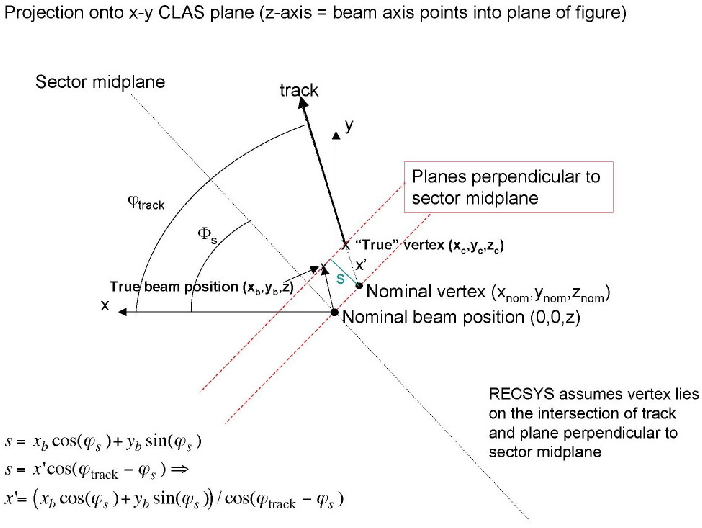
\epsfig{height=10cm,width=15cm,file=figuresEG4/FigKineCor/Raster_Corr_Formulae_Page_1.png}}
\caption{Raster correction geometry illustration (Figure courtesy of S. Kuhn)}
\label{fig:RstGeoKuhn1}
\end{figure}

The ADC values thus recorded can be translated to the coordinates (x,y) of the exact beam position at the target. The values of x,y can then be used to make corrections to the original track by RECSIS (which assumes x and y were zero), allowing better z-vertex and azimuthal angle ($\phi$) reconstruction. The better z-vertex reconstruction allows better selection of events from the target proper, rejecting events from upstream and downstream %up-beam and down-beam %GED
windows (especially for particles at small angles), and can also be used to reduce accidental coincidences in multi-particle final states (or to look for offset decays such as from $\Lambda$). Correction of $\phi$ improves missing mass resolution for multi-particle final states which is very important in exclusive channel analysis. In addition, plotting a two-dimensional histogram of events as a function of the raster information x and y, one can look for mis-steered beam that might have hit the target cup edges.

\begin{figure}[htpb] %ht, htpb (p - float, b = bottom, h=? t = top)
\centerline{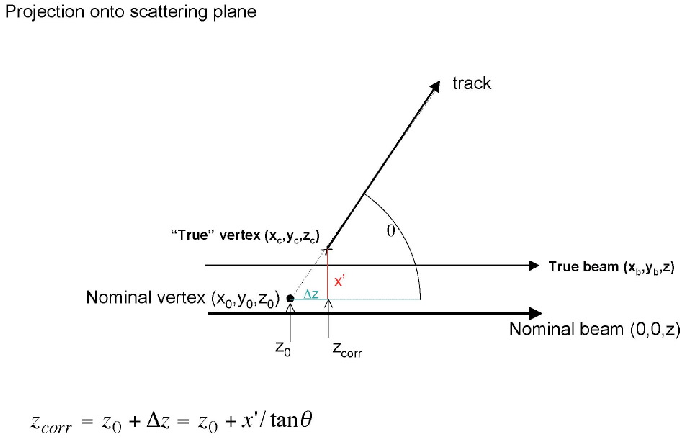
\epsfig{height=10cm,width=15cm,file=figuresEG4/FigKineCor/Raster_Corr_Formulae_Page_2.png}}
\caption{Raster correction geometry illustration (Figure courtesy - S. Kuhn)}
\label{fig:RstGeoKuhn2}
\end{figure}

A procedure was developed by P. Bosted \etal \cite{rstcor_cn} to translate the raster ADC values %counts 
into the beam coordinates x, y and then use them to improve the z-vertex and $\phi$ reconstruction. This procedure was successfully applied in previous CLAS experiments and EG4 has also embraced it to do the needed raster correction.


In short, the procedure for this correction is as follows: %does the following:
\begin{enumerate}
\item Translates raster-ADC values to beam coordinates x and y.
\item Corrects the event vertex z-coordinate (represented as v$_z$ in the data). %pass1 ntuples) %SEK
\item Corrects the azimuthal angle $\phi$ of each particle in the event.
\end{enumerate} 

% new paragraph \\
This correction is applied before the momentum correction. So, the partially corrected $\phi$ and v$_z$ will be a part 
of the input fed into the next stage of the kinematic correction which, henceforth, will be termed ``momentum correction''.



%\subsection{Procedure to translate ADC counts to beam positions x and y (in centimeters)}
\subsubsection{Procedure to translate ADCs to centimeters}

\begin{figure}[htpb] %ht, htpb (p - float, b = bottom, h=? t = top)
\centerline{\epsfig{height=10cm,width=10cm,file=figuresEG4/FigKineCor/Rst21pCorXY.png}}  %kp: Disabled for Suman Jee's trimming test (enable back)
%\centerline{\includegraphics[trim = 0mm 0mm 0mm 50mm, clip = true, scale = 0.5] {chap7KineCor/figures/Rst21pCorXY.png}} %7/27/12
\caption{Beam coordinates x and y calculated with the raster correction procedure.}
\label{fig:RstXY}
\end{figure}

The procedure assumes that a linear relation holds between the raster currents and the beam coordinates x and y (displacements %bendings 
in cm produced by the field of the currents) as follows:

\begin{subequations}
\label{eqRC-Adc2cm}
\begin{eqnarray}
\label{eqRC-Adc2cm1}
x = (X_{adc}-X_{offset})C_x,
\end{eqnarray}

\begin{eqnarray}
\label{eqRC-Adc2cm2}
y = (Y_{adc}-Y_{offset})C_y,
\end{eqnarray}
\end{subequations}
where, $X_{offset}$, $Y_{offset}$, $C_x$, and $C_y$ are the %constants/
parameters to be determined by the procedure. These parameters are determined by selecting reasonably well reconstructed events each consisting of more than one charged  particles tracks originating reasonably close to the nominal target center (v$_z \approx $- 101.0 cm) and using them in TMinuit (ROOT Minuit program) to minimize the $\chi^2$, defined as
\begin{eqnarray}
\label{eqRC-chiSq}
\chi^2 = \sum^N_{i=1}((z_{corr})_i - z_o)^2,
\end{eqnarray}
where $z_0$ is the 5th parameter that defines the center of the target and is to be determined from the minimization. %/fitting. 
Likewise, $z_{corr}$ is the trial value of the corrected z-vertex (a function of trial values of the first four fit parameters, as will be evident below). TMinuit will give us those values of the parameters which gives 
the $\chi^2$ a minimum value.

\begin{comment}
\begin{figure}[h] %ht, htpb (p - float, b = bottom, h=? t = top)
\centerline{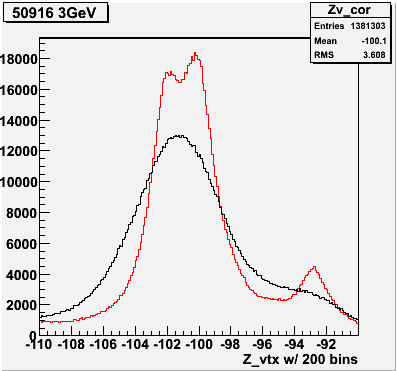
\epsfig{height=15cm,width=15cm,file=figuresEG4/FigKineCor/MTc3G50916one.png}}
\caption[Vz from Empty target run]{Vertex Z-coordinates of scattered electrons from an 3.0 GeV empty-cell-target run}
\label{fig:MTcellVz1}
\end{figure}
\end{comment}

\begin{figure}[h] 
\centering
  \leavevmode 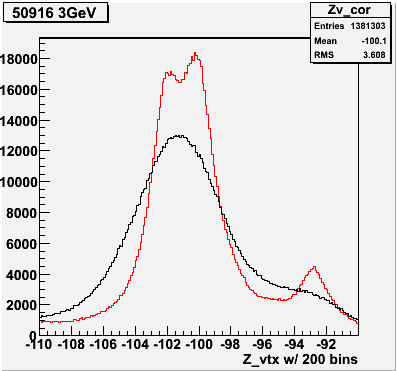
\includegraphics[width=0.8\textwidth]{figuresEG4/FigKineCor/MTc3G50916one.png}   
  \caption[Vz from Empty target run]{Vertex Z-coordinates (in cm) of scattered electrons from an 3.0 GeV empty-cell-target run before (black) and after (red) the raster corrections. It is clear that the correction improves the resolution, thus revealing the positions of the empty target cells (the first two peaks near -101.0 cm) and the heat shield (around -93.0 cm).}
  \label{fig:MTcellVz1}
\end{figure}



From a simple geometry consideration (as illustrated in Figs. \ref{fig:RstGeoKuhn1} and \ref{fig:RstGeoKuhn2}), an expression for correction to the z-vertex in terms of x, y and angles of a particle track is arrived at as follows:
\begin{eqnarray}
\label{eqRC-zcor}
z_{corr} = z_{recsis} + x'/tan(\theta),
\end{eqnarray}
where $z_{recsis}$, and $z_{corr}$ are the z-vertex measured %/reconstructed 
by the tracking code and the raster-corrected z-vertex respectively, and
\begin{eqnarray}
\label{eqRC-xprime}
x' = (x~cos\phi_s + y~sin\phi_s)/cos(\phi - \phi_s),
\end{eqnarray}
is the distance in cm along the track length that was not considered in tracking (because the tracking code assumes that the track started from $x = 0$, $y = 0$); $\phi_s$ is the sector angle defined as the azimuthal angle of the sector mid-plane (equal to $(s-1 \cdot 60$ degrees, where $s$ is the sector number from 1 to 6), and $\phi$ is the azimuthal angle of the particle (in the lab-coordinate system) defined as $\phi = arctan(cy/cx)$, %atan2(cy,cx), atan2 is a programming jargon, just write "arctan" %SEK
where $cx$ and $cy$ are the x- and y- direction cosines of the track. 

Due to the difference of the actual track length (through the 50 kG magnetic field of the target) from what is assumed by the tracking software, the azimuthal angle \phs is reconstructed incorrectly. The angle \phs can now be corrected by adding a correction term $- 50 q (x'/100)/33.356/p_t$ to the reconstructed value $\phi_{recsis}$ as follows:
\begin{eqnarray}
\label{eqRC-phcor}
\phi_{corr} = \phi_{recsis} - 50 q (x'/100)/33.356/p_t,
\end{eqnarray}
where $\phi_{recsis}$ and $\phi_{corr}$ are the reconstructed and corrected values of \phs respectively, $q$ is the particle charge in units of $e$, the factor 50 is the target field expressed in kG, the factor 100 is to convert the unit cm of $x'$ to m, the factor 33.356 is the inverse speed of light in the appropriate units and $p_t=p sin(\theta)$ is the particle's transverse momentum expressed in GeV \cite{rstcor_cn}.

% =====   12/5/13
For our analysis, all the four parameters $X_{offset}$, $Y_{offset}$, $C_x$, and $C_y$ were determined separately for each beam energy by selecting a set of good electrons and using the method of $\chi^2$ minimization (see Eq. \ref{eqRC-chiSq}). With the parameters known, we can use Eqs. \ref{eqRC-Adc2cm1} and \ref{eqRC-Adc2cm} to convert the X- and Y- ADC values into beam positions (at the target location) in centimeters as shown in Fig. \ref{fig:RstXY} for 1.3 GeV data. Likewise,  $vz$ and \phs can be corrected by calculating the correction terms $x'/tan(\theta)$ and $- 50 q (x'/100)/33.356/p_t$ and adding them to the respective reconstructed values (see Eqs. \ref{eqRC-zcor}, \ref{eqRC-phcor}). For example, Fig. \ref{fig:MTcellVz1} shows the distribution of electron Z-vertex distribution (from 3 GeV proton data) before and after the corrections. It is evident from the figure that the corrections improves the resolution as expected in addition to shifting (towards left) the average position of the distribution by some amount.
%\textcolor{red}{SEK: Section missing: What is the actual correction on Z, \ph? also, comment on result of fit procedure Fig. \ref{fig:RstXY}, and how it is applied to Zcor. }
